\documentclass{beamer}

\usepackage{beamerthemesplit}
\usepackage{amsmath}
\usepackage{amsfonts}
\usepackage{amssymb}
\usepackage{qtree}
\usepackage{cancel}
\usepackage{tkz-graph}
%\usepackage[pdftex]{graphicx}

\mode<presentation>
{
  \usetheme{Warsaw}
  % or ...

  %\setbeamercovered{transparent}
  % or whatever (possibly just delete it)
}


\usepackage[english]{babel}
% or whatever

\usepackage[latin1]{inputenc}
% or whatever

\usepackage{times}
\usepackage[T1]{fontenc}

\title{Probabilistic Logical Networks}

\subtitle{Intensional Inference}

\author{Nil Geisweiller}

\institute[Xiamen University] % (optional, but mostly needed)
{
  Novamente LLC
}

\date[Xiamen University AGI Summer School 2009] % (optional, should be abbreviation of conference name)
{Xiamen University\\ AGI Summer School 2009}


\AtBeginSection[]
{
  \begin{frame}<beamer>{Outline}
    \tableofcontents[currentsection,currentsection]
  \end{frame}
}

\AtBeginSubsection[]
{
  \begin{frame}<beamer>{Outline}
    \tableofcontents[currentsection,currentsubsection]
  \end{frame}
}

%\newcommand{\AND}{\textit{AND}}
%\newcommand{\OR}{\textit{OR}}
%\newcommand{\NOT}{\textit{NOT}}
\newcommand{\AND}{\land}
\newcommand{\OR}{\lor}
\newcommand{\NOT}{\lnot}


\begin{document}

\frame
{
  \maketitle
}
\section[Outline]{}
\frame{\tableofcontents}

\section{Extensionality vs Intensionality}

\frame
{
  \frametitle{Intensionality vs Extensionality}

  \begin{columns}
    \column{1.5in}
    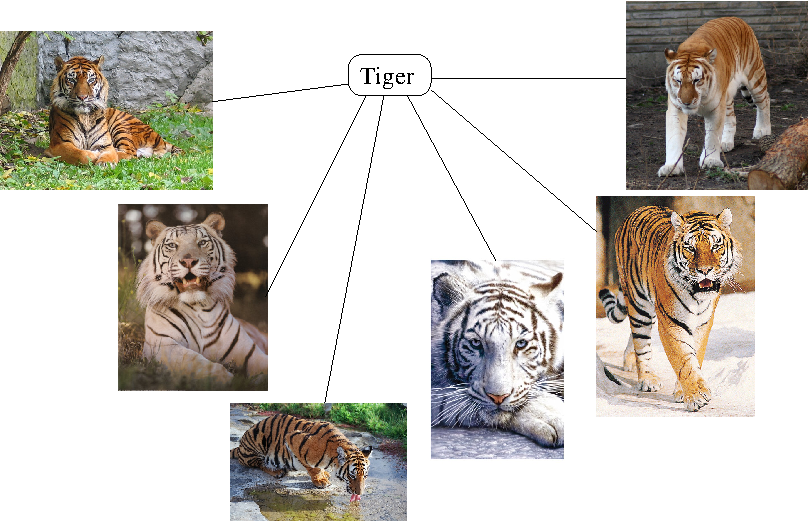
\includegraphics[scale=0.3]{extension_tiger.pdf}\\
    \alert{Extension} of a term: set of \alert{objects}

    \column{1.5in}

    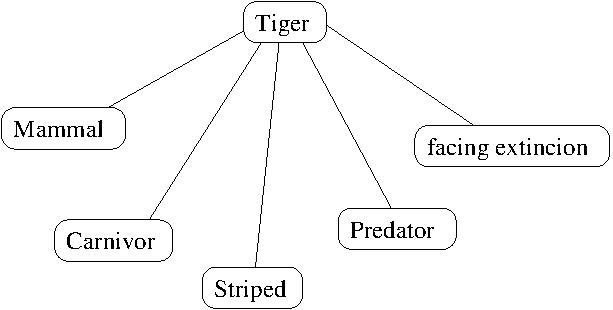
\includegraphics[scale=0.4]{intension_tiger.pdf}\\
    \alert{Intension} of a term: set of \alert{properties}
  \end{columns}

%   \begin{itemize}
%   \item \alert{Extension} of a term: set of \alert{objects}
%   \item 
%   \end{itemize}

}

\frame[containsverbatim]
{
  \frametitle{Intensionality vs Extensionality}
  \begin{beamerboxesrounded}{definition}
    \begin{itemize}
    \item ExtInh = ExtensionalInheritanceLink
    \item IntInh = IntensionalInheritanceLink
    \end{itemize}
  \end{beamerboxesrounded}

  \begin{columns}
    \column{1.5in}

    {\footnotesize
      {\tt
        \begin{itemize}
        \item 
          ExtInh<1>\\
          $\ \ \ \ ${\color{green} Siberian\_Tiger}\\
          $\ \ \ \ ${\color{blue} Tiger}\\
        \item
          ExtInh<1>\\
          $\ \ \ \ ${\color{red} Xiamen\_tiger}\\
          $\ \ \ \ ${\color{blue} Tiger}\\
        \item
          ExtInh<0>\\
          $\ \ \ \ ${\color{brown} Lion}\\
          $\ \ \ \ ${\color{blue} Tiger}\\
        \end{itemize}
      }
    }

    \column{1.5in}
    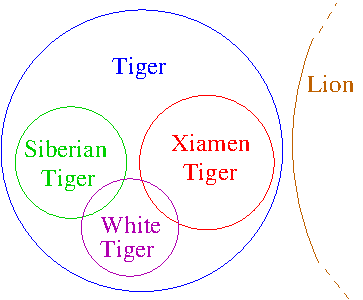
\includegraphics[scale=0.5]{tiger_set.pdf}
  \end{columns}
}

\frame[containsverbatim]
{
  \frametitle{Intensionality vs Extensionality}

  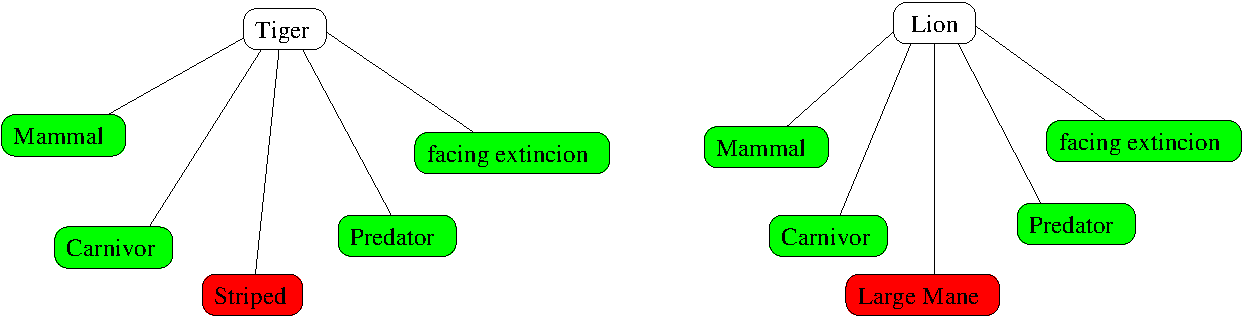
\includegraphics[scale=0.5]{intinh_tiger_lion.pdf}

  \begin{beamerboxesrounded}{Lion Inherits Tiger Intensionally}
  Tiger and Lion share many properties:
%    {\footnotesize
\begin{verbatim}
IntInh<0.78>
    Lion
    Tiger
\end{verbatim}
%    }
\end{beamerboxesrounded}

}

\frame[containsverbatim]
{
  \frametitle{Mixed Inheritance}

  \begin{beamerboxesrounded}{Mixed Inheritance}
    Disjunction of Extensional and Intensional Inheritance.
    \\[2ex]

  {\tt
    Inheritance A B <tv>}\\[2ex]
  $\equiv$
\begin{verbatim}
OR<tv>
    ExtInh A B
    IntInh A B
\end{verbatim}
  \end{beamerboxesrounded}
}

\section{Extensional Inheritance}

\frame
{
  \frametitle{Extensional Inheritance $\equiv$ SubSet}

  \begin{columns}
    \column{1.5in}
    
    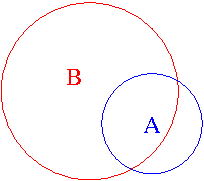
\includegraphics[scale=0.7]{subset_A_B.pdf}

    \column{1.5in}

    \visible<2>{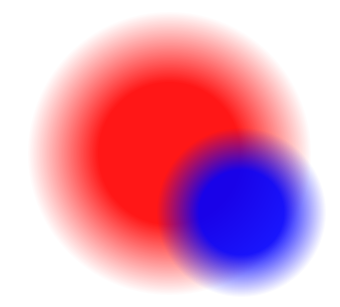
\includegraphics[scale=0.25]{Fuzzy_SubSet_A_B.png}}

  \end{columns}

  {\tt ExtInh {\color{blue}A} {\color{red}B} <p>
    $\ \equiv\ $
    {\tt SubSet {\color{blue}A} {\color{red}B} <p>}
    $\ \equiv\ P({\color{red}B}|{\color{blue}A})=p$}\\[2ex]

  \pause

  \begin{itemize}
  \item
    Fuzzy set $\Rightarrow$ heuristic to compute 
    $P({\color{red}B}|{\color{blue}A})$
  \end{itemize}

  \begin{eqnarray*}
    P({\color{red}B}|{\color{blue}A})
    &
    =
    &
    \frac{\sum_x \min({\color{blue}A}(x), {\color{red}B}(x))}
    {\sum_x {\color{blue}A}(x)}
  \end{eqnarray*}

}

\section{Intensional Inheritance}

\frame
{
  \frametitle{What is a property?}

  \begin{center}
    %\alert{
      Property = Super-set
    %}

      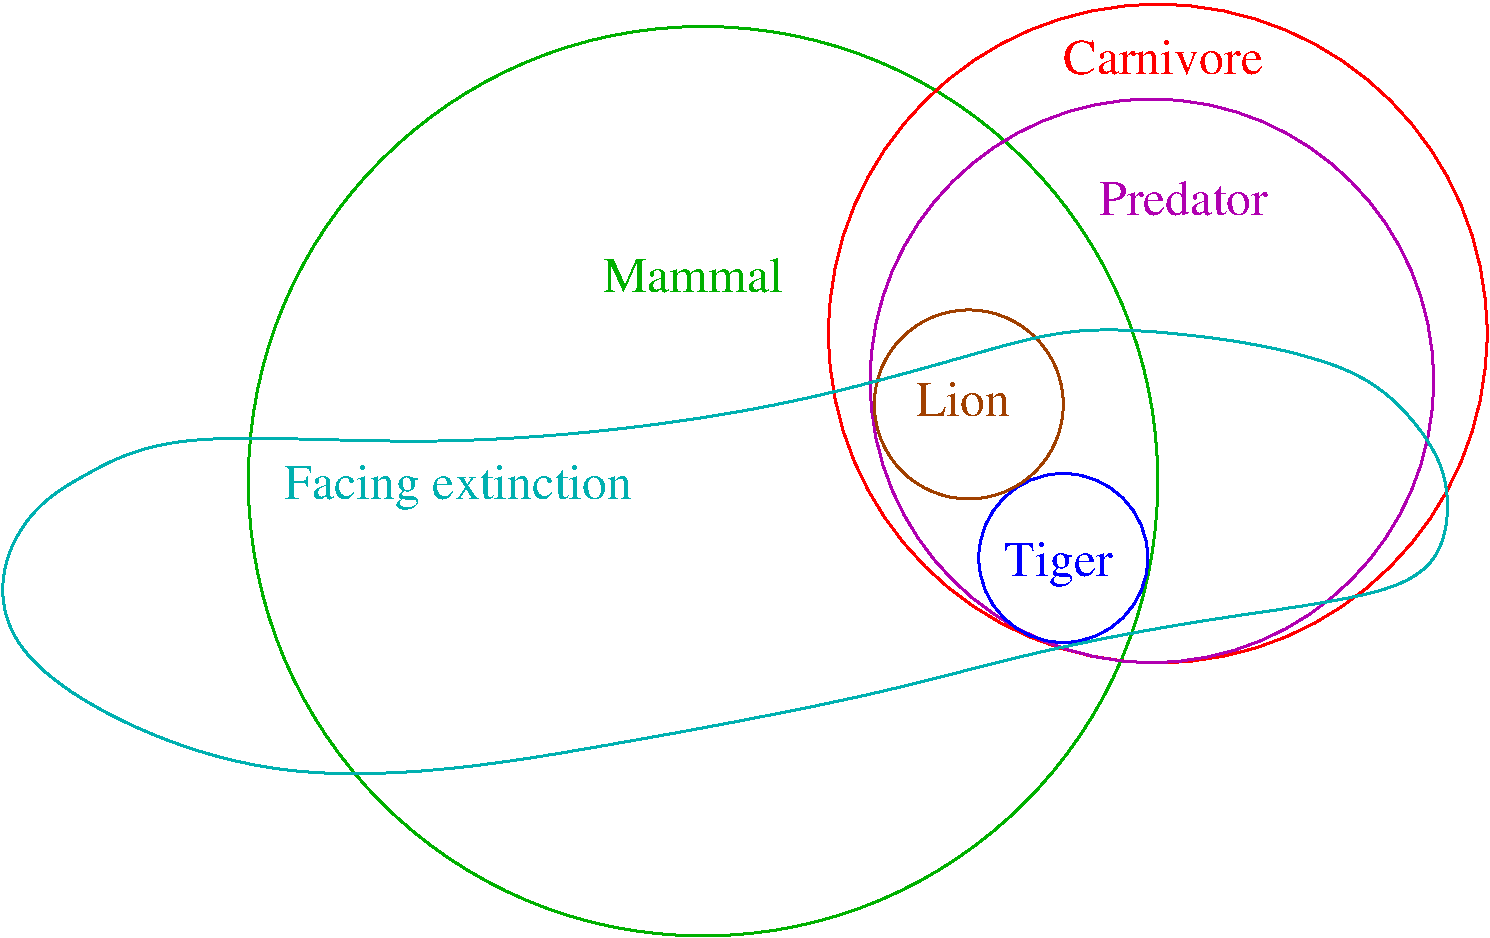
\includegraphics[scale=0.35]{property_superset.pdf}
  
  \end{center}

%   \pause

%   \begin{itemize}
%   \item<+-> Properties of Tiger: Predator,
%  Carnivore, Facing extinction, Mammal
%   \end{itemize}
}

\frame
{
  \frametitle{What is a property?}

  \begin{columns}

    \column{2in}
    
    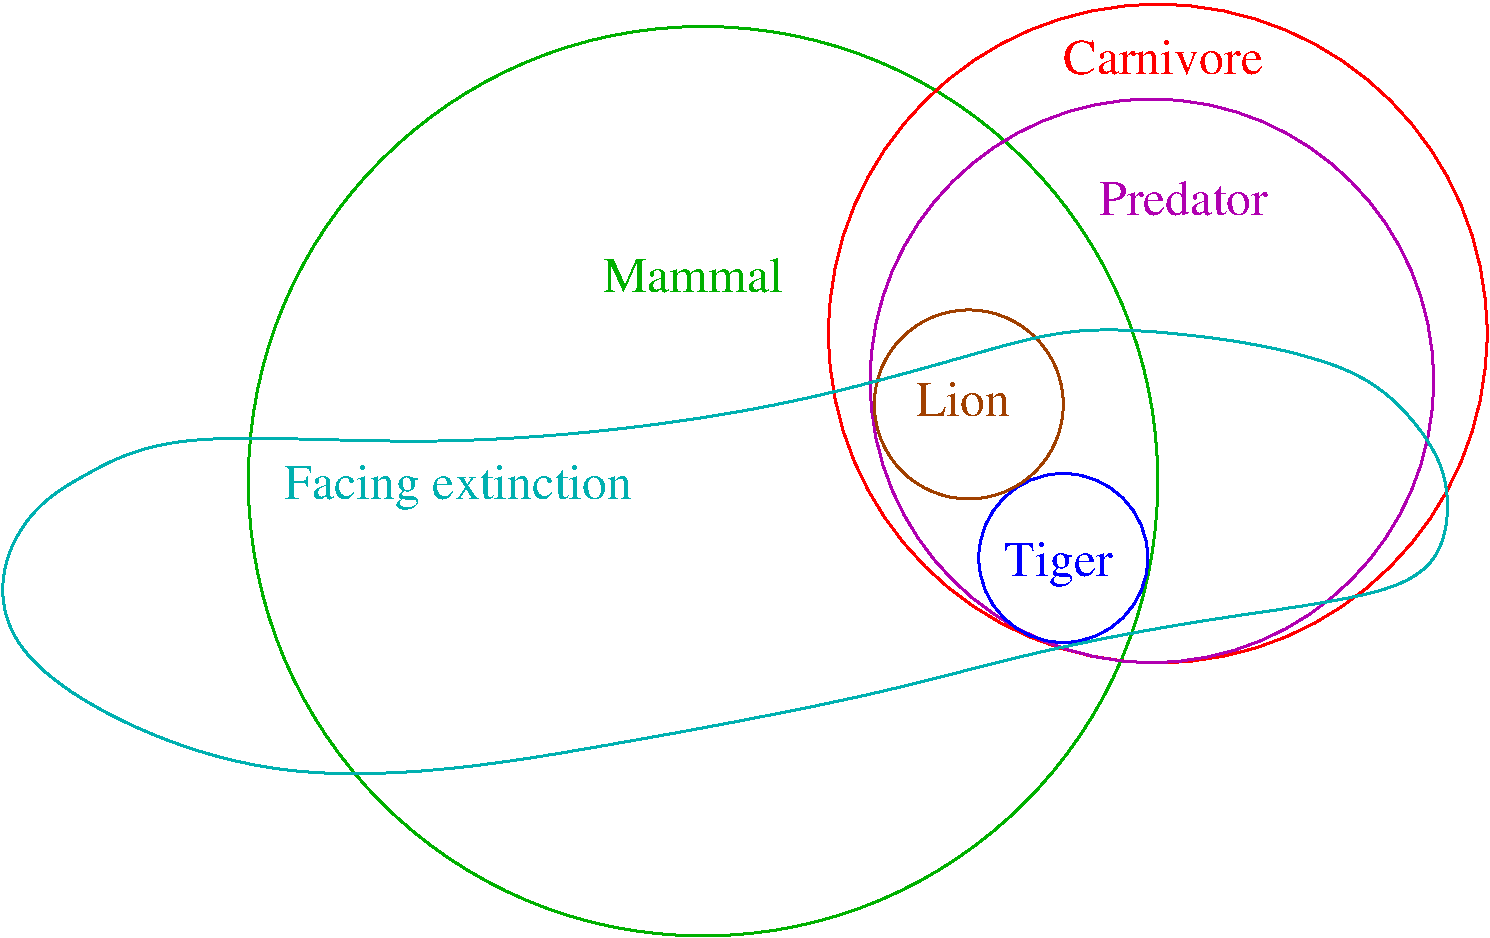
\includegraphics[scale=0.2]{property_superset.pdf}
    
    \column{2in}
  
    {\footnotesize
      \begin{itemize}
      \item {\tt SubSet {\color{blue}T} {\color{cyan}Fe} <1>}
      \item {\tt SubSet {\color{blue}T} {\color{purple}P} <1>}
      \item {\tt SubSet {\color{blue}T} {\color{red}C} <1>}
      \item {\tt SubSet {\color{blue}T} {\color{green}M} <1>}
      \item {\tt SubSet {\color{brown}L} {\color{cyan}Fe} <0.8>}
      \item {\tt SubSet {\color{brown}L} {\color{blue}T} <0>}
      \end{itemize}
    }
  \end{columns}

   \pause

   \begin{columns}

     \column{1.3in}

     {\footnotesize
     \begin{itemize}
     \item $P({\color{cyan}Fe}|{\color{blue}T})=1$
     \item $P({\color{purple}P}|{\color{blue}T})=1$
     \item $P({\color{red}C}|{\color{blue}T})=1$
     \item $P({\color{green}M}|{\color{blue}T})=1$
     \item $P({\color{cyan}Fe}|{\color{brown}L})=0.8$
     \item $P({\color{blue}T}|{\color{brown}L})=0$
     \end{itemize}
     }

     \pause

     \column{0.2in}

     $\Rightarrow$

     \column{2in}

     \begin{beamerboxesrounded}{$F$ is a \alert{property} of $G$ if}
       \alert{$P(F|G)$} is sufficiently \alert{high}
     \end{beamerboxesrounded}

   \end{columns}
}

\frame
{
  \frametitle{What is an \alert{interesting} property?}

  But potentially$\ldots$
  \alert{infinity of super-sets} (i.e. properties) of a term\\[5ex]

  \begin{beamerboxesrounded}{Interesting property of a term}
    \begin{enumerate}
    \item Help \alert{differentiate} that term
    \item \alert{Less complex} than the term itself
    \end{enumerate}
  \end{beamerboxesrounded}
}

\frame
{
  \frametitle{Interesting property: help \alert{differentiate}}

  %Example with the property 
  \alert{$being\_part\_of\_the\_universe$}\\
  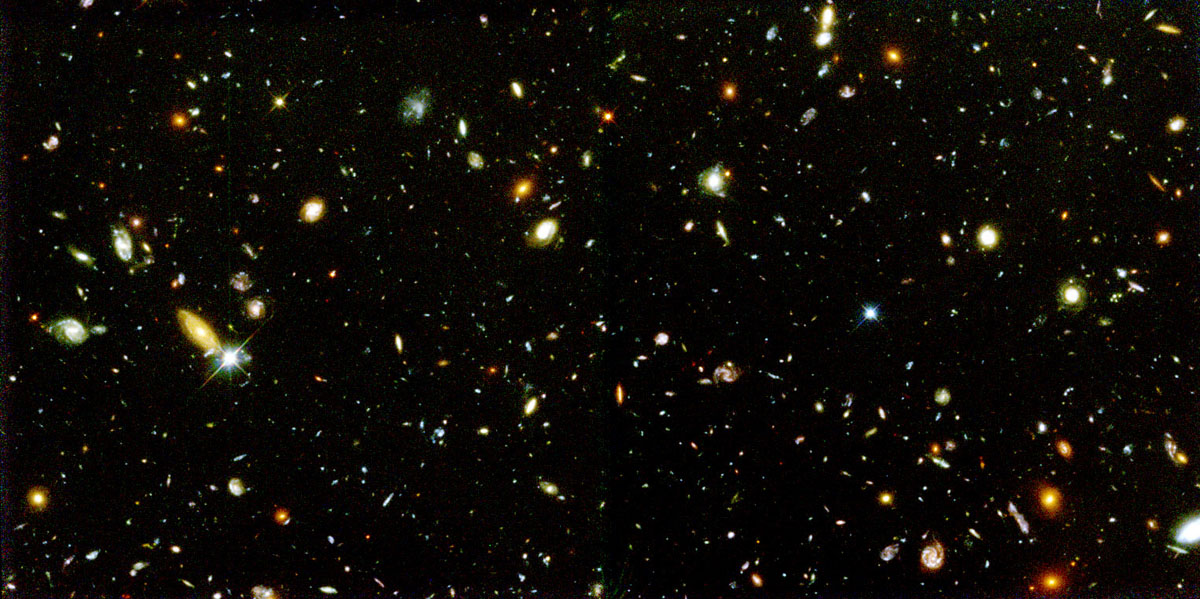
\includegraphics[scale=0.12]{universe.jpg}

  $P(being\_part\_of\_the\_universe|Tiger)=1$\\
  $P(being\_part\_of\_the\_universe|Lion)=1$\\
  $P(being\_part\_of\_the\_universe|Chair)=1$\\
  $\ldots$\\

  \pause

  \begin{beamerboxesrounded}{being\_part\_of\_the\_universe
      \alert{not interesting property} of Tiger}
    because it does not help to differentiate it in any manner
  \end{beamerboxesrounded}
}

\frame
{
  \frametitle{Interesting property: help \alert{differentiate}}

  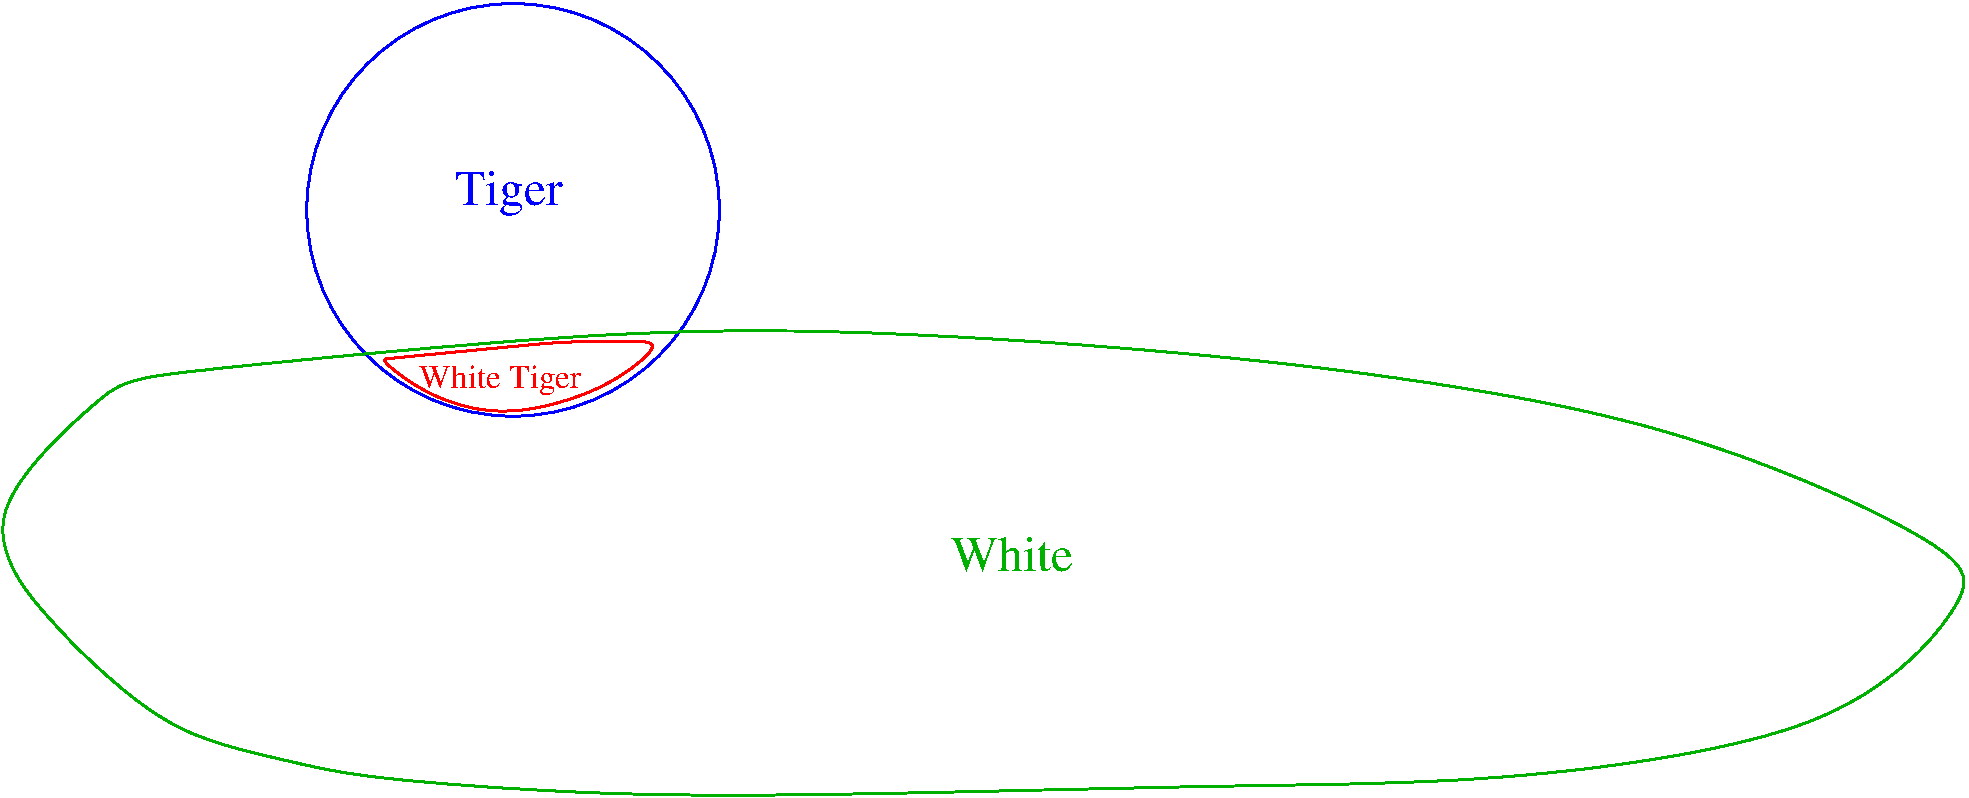
\includegraphics[scale=0.32]{white_tiger.pdf}

  \begin{beamerboxesrounded}{White is an
      \alert{interesting property} of White\_Tiger}
    \begin{itemize}
    \item $P({\color{green}White}|{\color{red}White\_Tiger})=1$
    \item $P({\color{green}White}|Golden\_Tiger)=0$
%    \item $White\ AND\ Tiger = White\_Tiger$
    \end{itemize}
  \end{beamerboxesrounded}
 
}

\frame
{
  \frametitle{Interesting property: help \alert{differentiate}}

  \begin{beamerboxesrounded}{$F$ helps \alert{differentiate} $G$,
      or $F$ is \alert{associated} with $G$ iff}
    $P(F|G) > P(F|\lnot G)$
  \end{beamerboxesrounded}
  
  \[ASSOC(F,G) = [P(F|G)-P(F|\lnot G)]^+\]

  \pause

  Examples
  \begin{enumerate}
  \item<+-> 
    $\alert{ASSOC(being\_part\_of\_the\_universe, Tiger)}$\\
    $
    \begin{array}{clrl}
      = & & [ & P(being\_part\_of\_the\_universe|Tiger)\\
      & &  & - P(being\_part\_of\_the\_universe|\lnot Tiger)]^+\\
      = & [1-1]^+ & = & \alert{0}\\
    \end{array}
    $
  \item<+->
    $\alert{ASSOC(White,White\_Tiger)}$\\
    $
    \begin{array}{cl}
      = & [ P(White|White\_Tiger) - P(White|\lnot White\_Tiger)]^+\\
      = & [ 1 - 0.3 ]^+ = \alert{0.7}
    \end{array}
    $
  \end{enumerate}

}

\frame
{
  \frametitle{Interesting property: \alert{Less complex} than the term itself}
  
  \only<1>{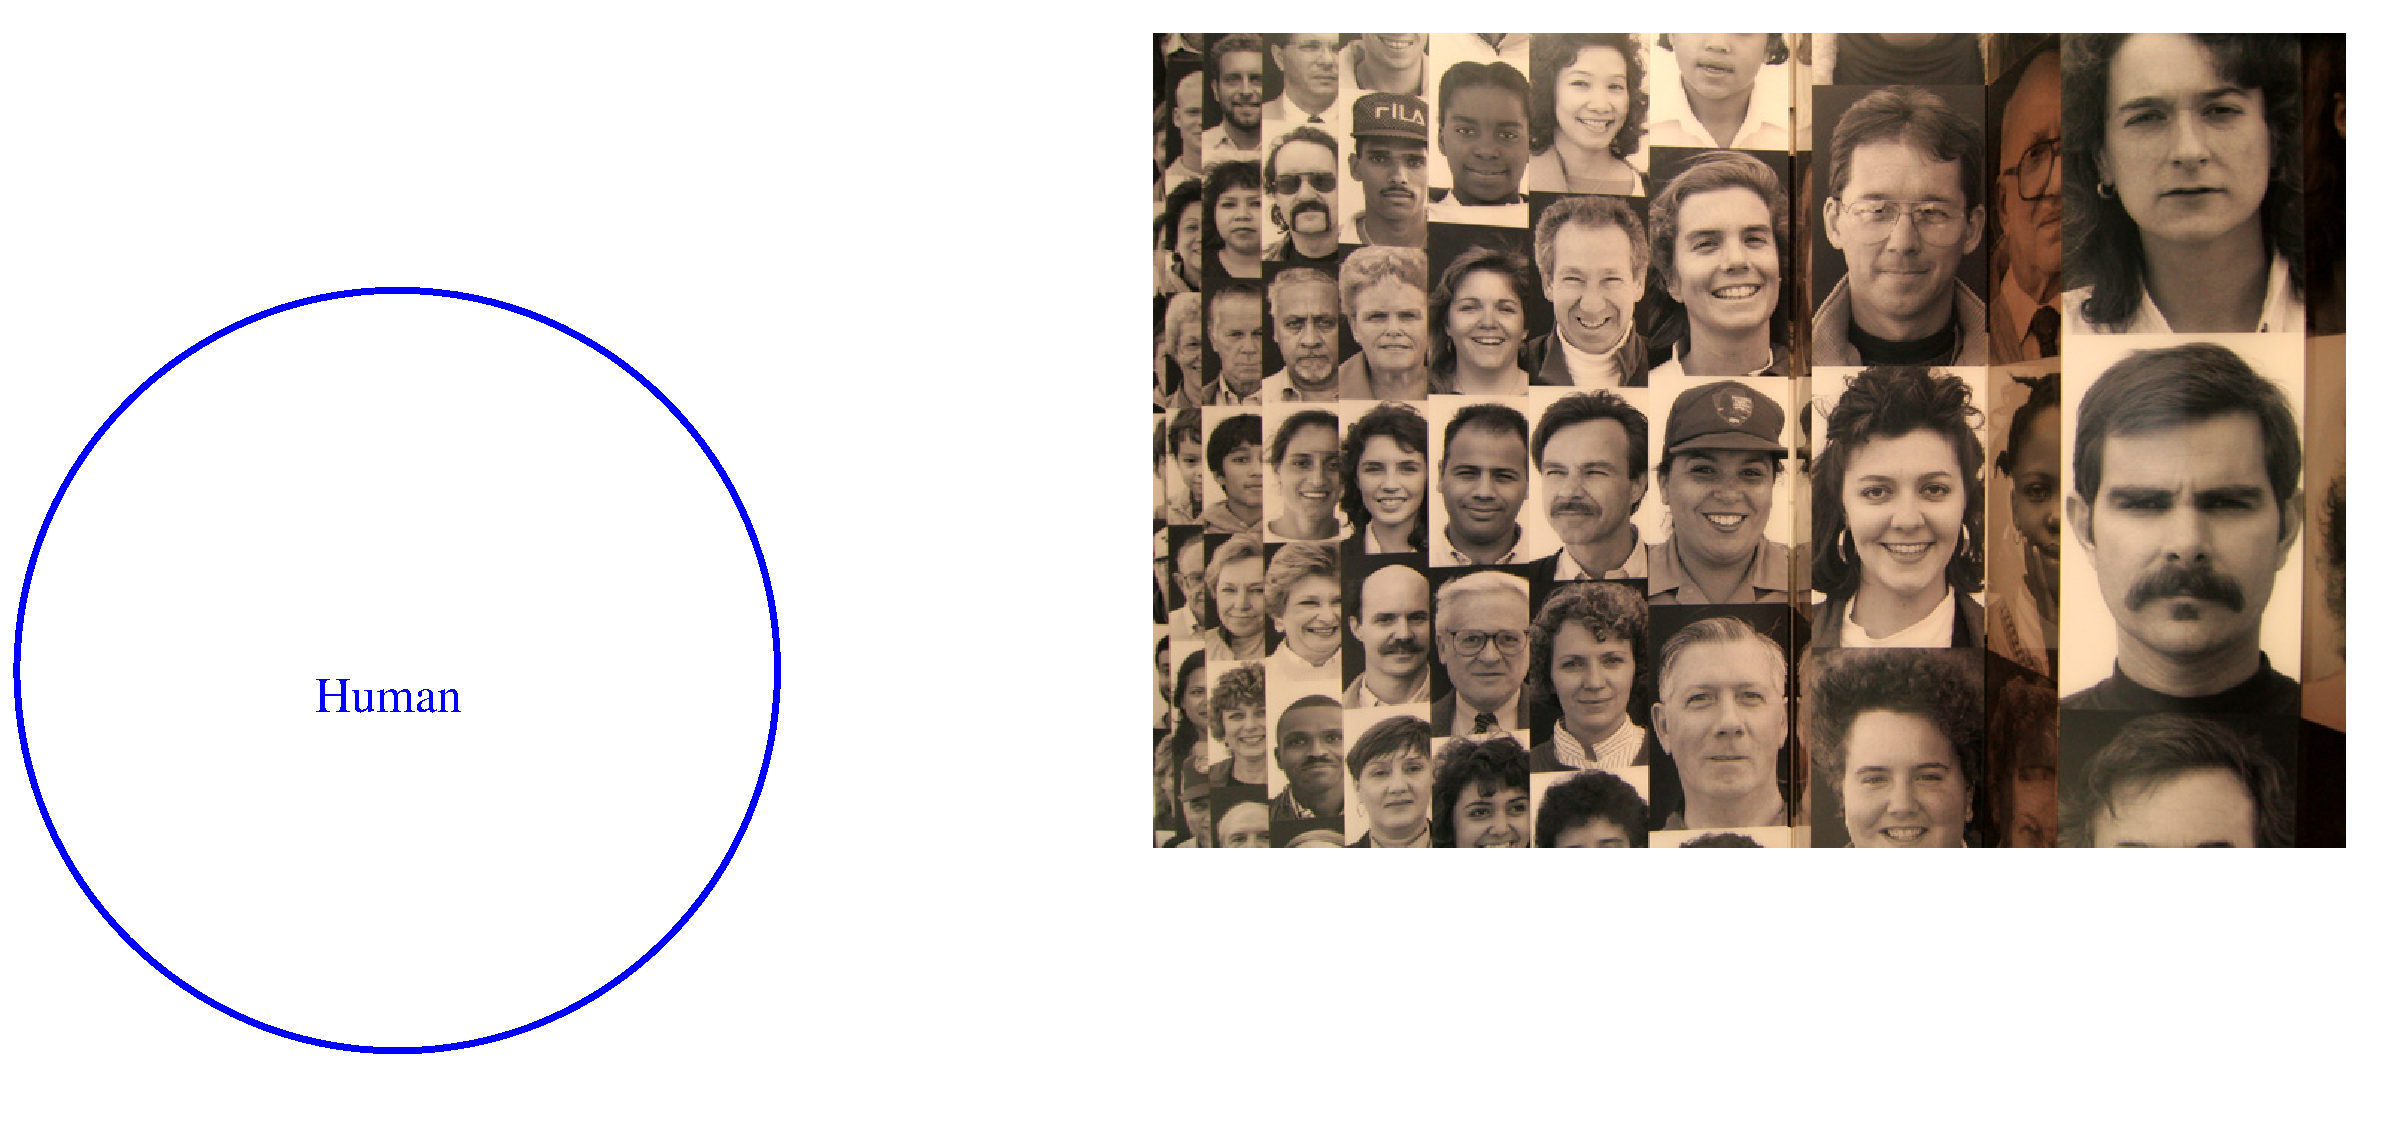
\includegraphics[scale=0.25]{human_chair_pic1.pdf}}
  \only<2>{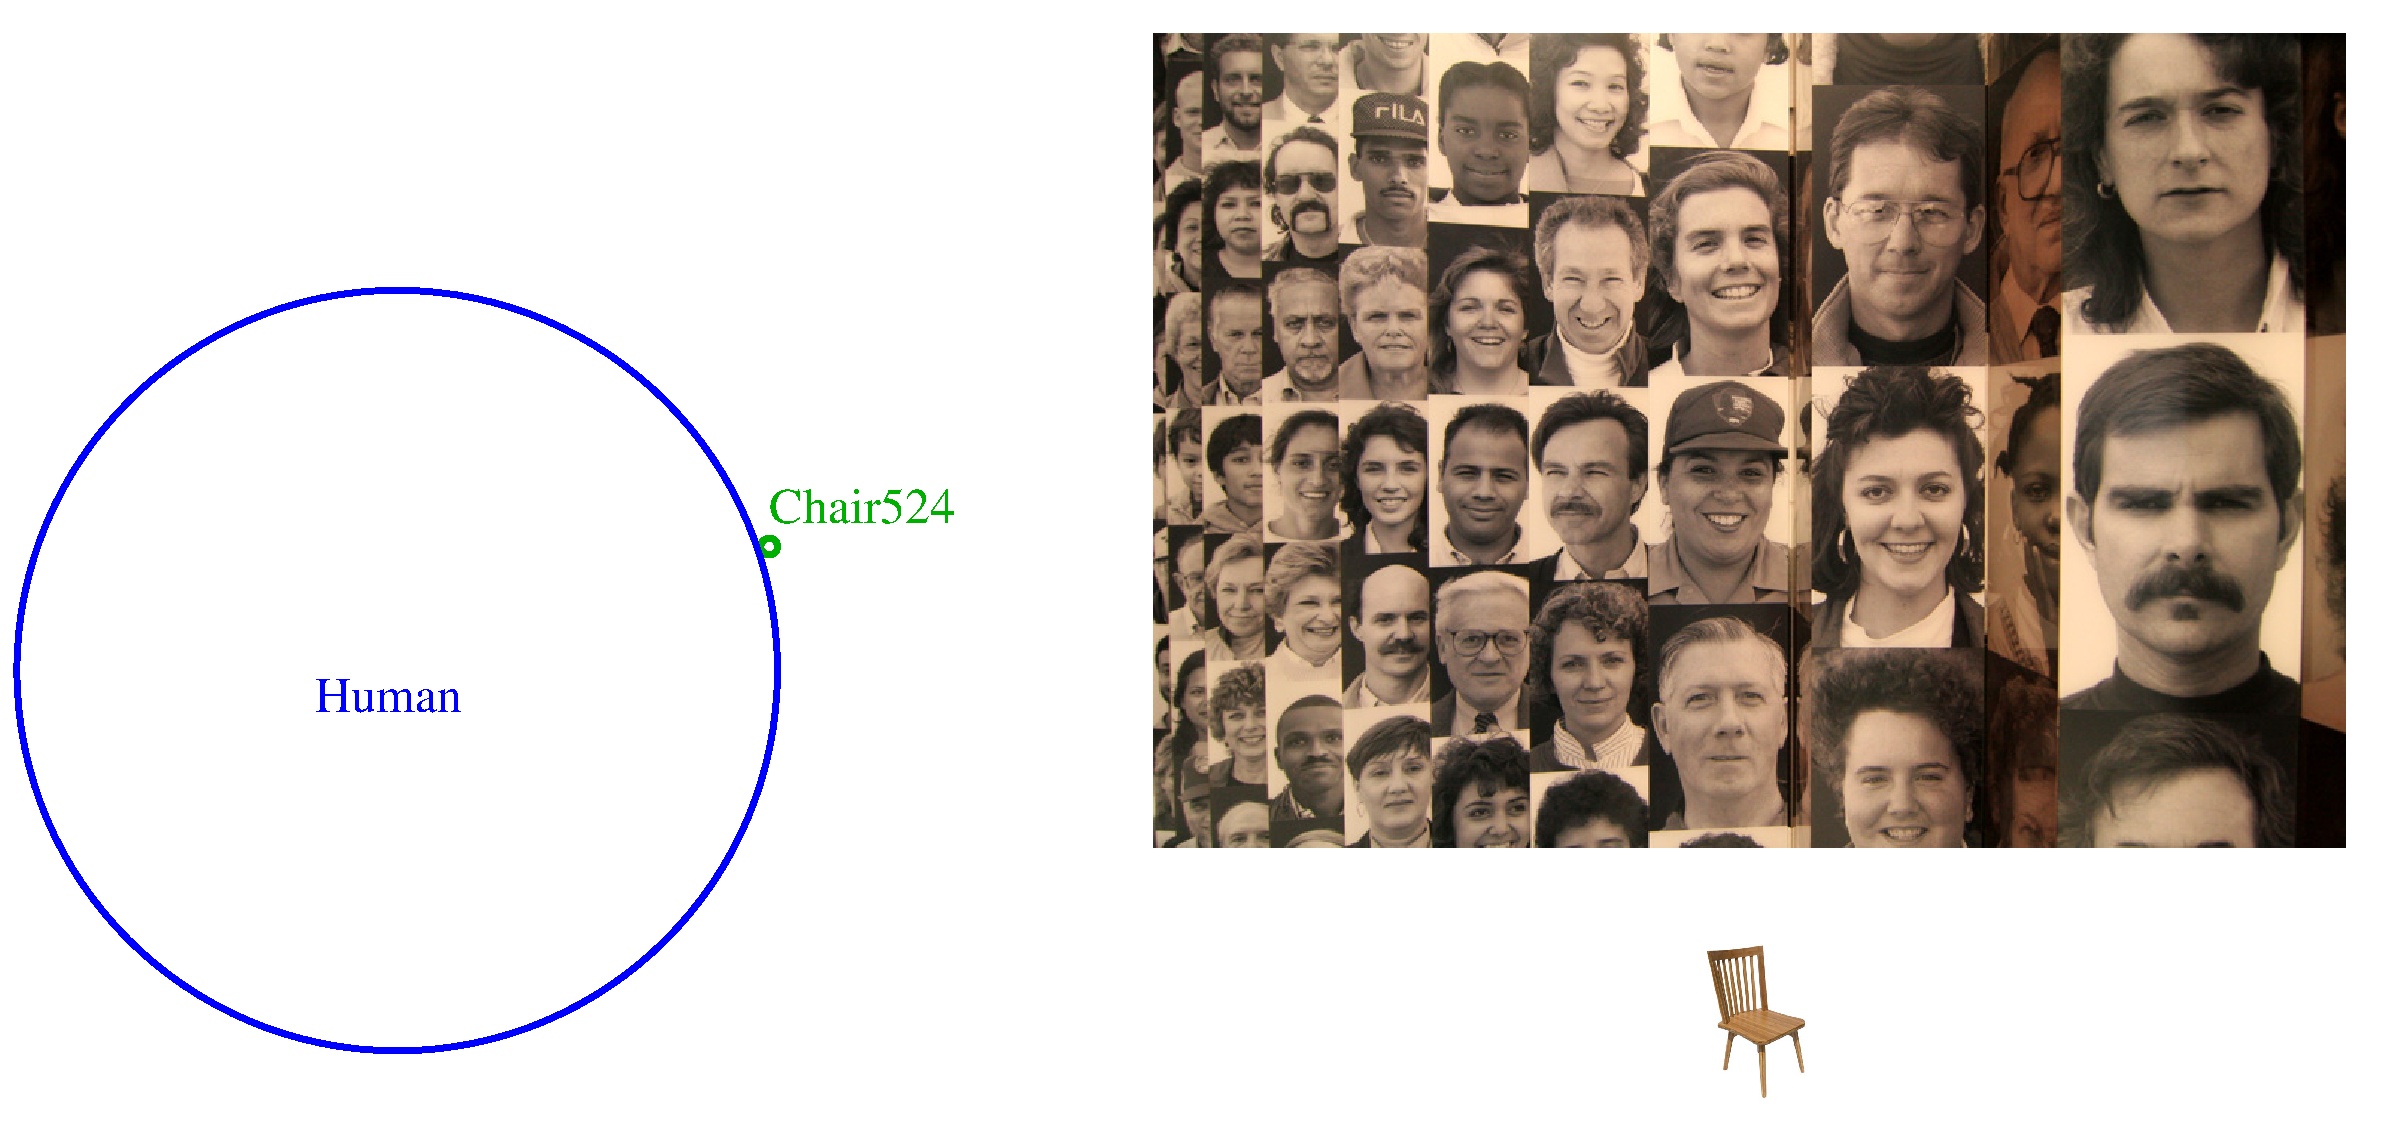
\includegraphics[scale=0.25]{human_chair_pic2.pdf}}
  \only<3->{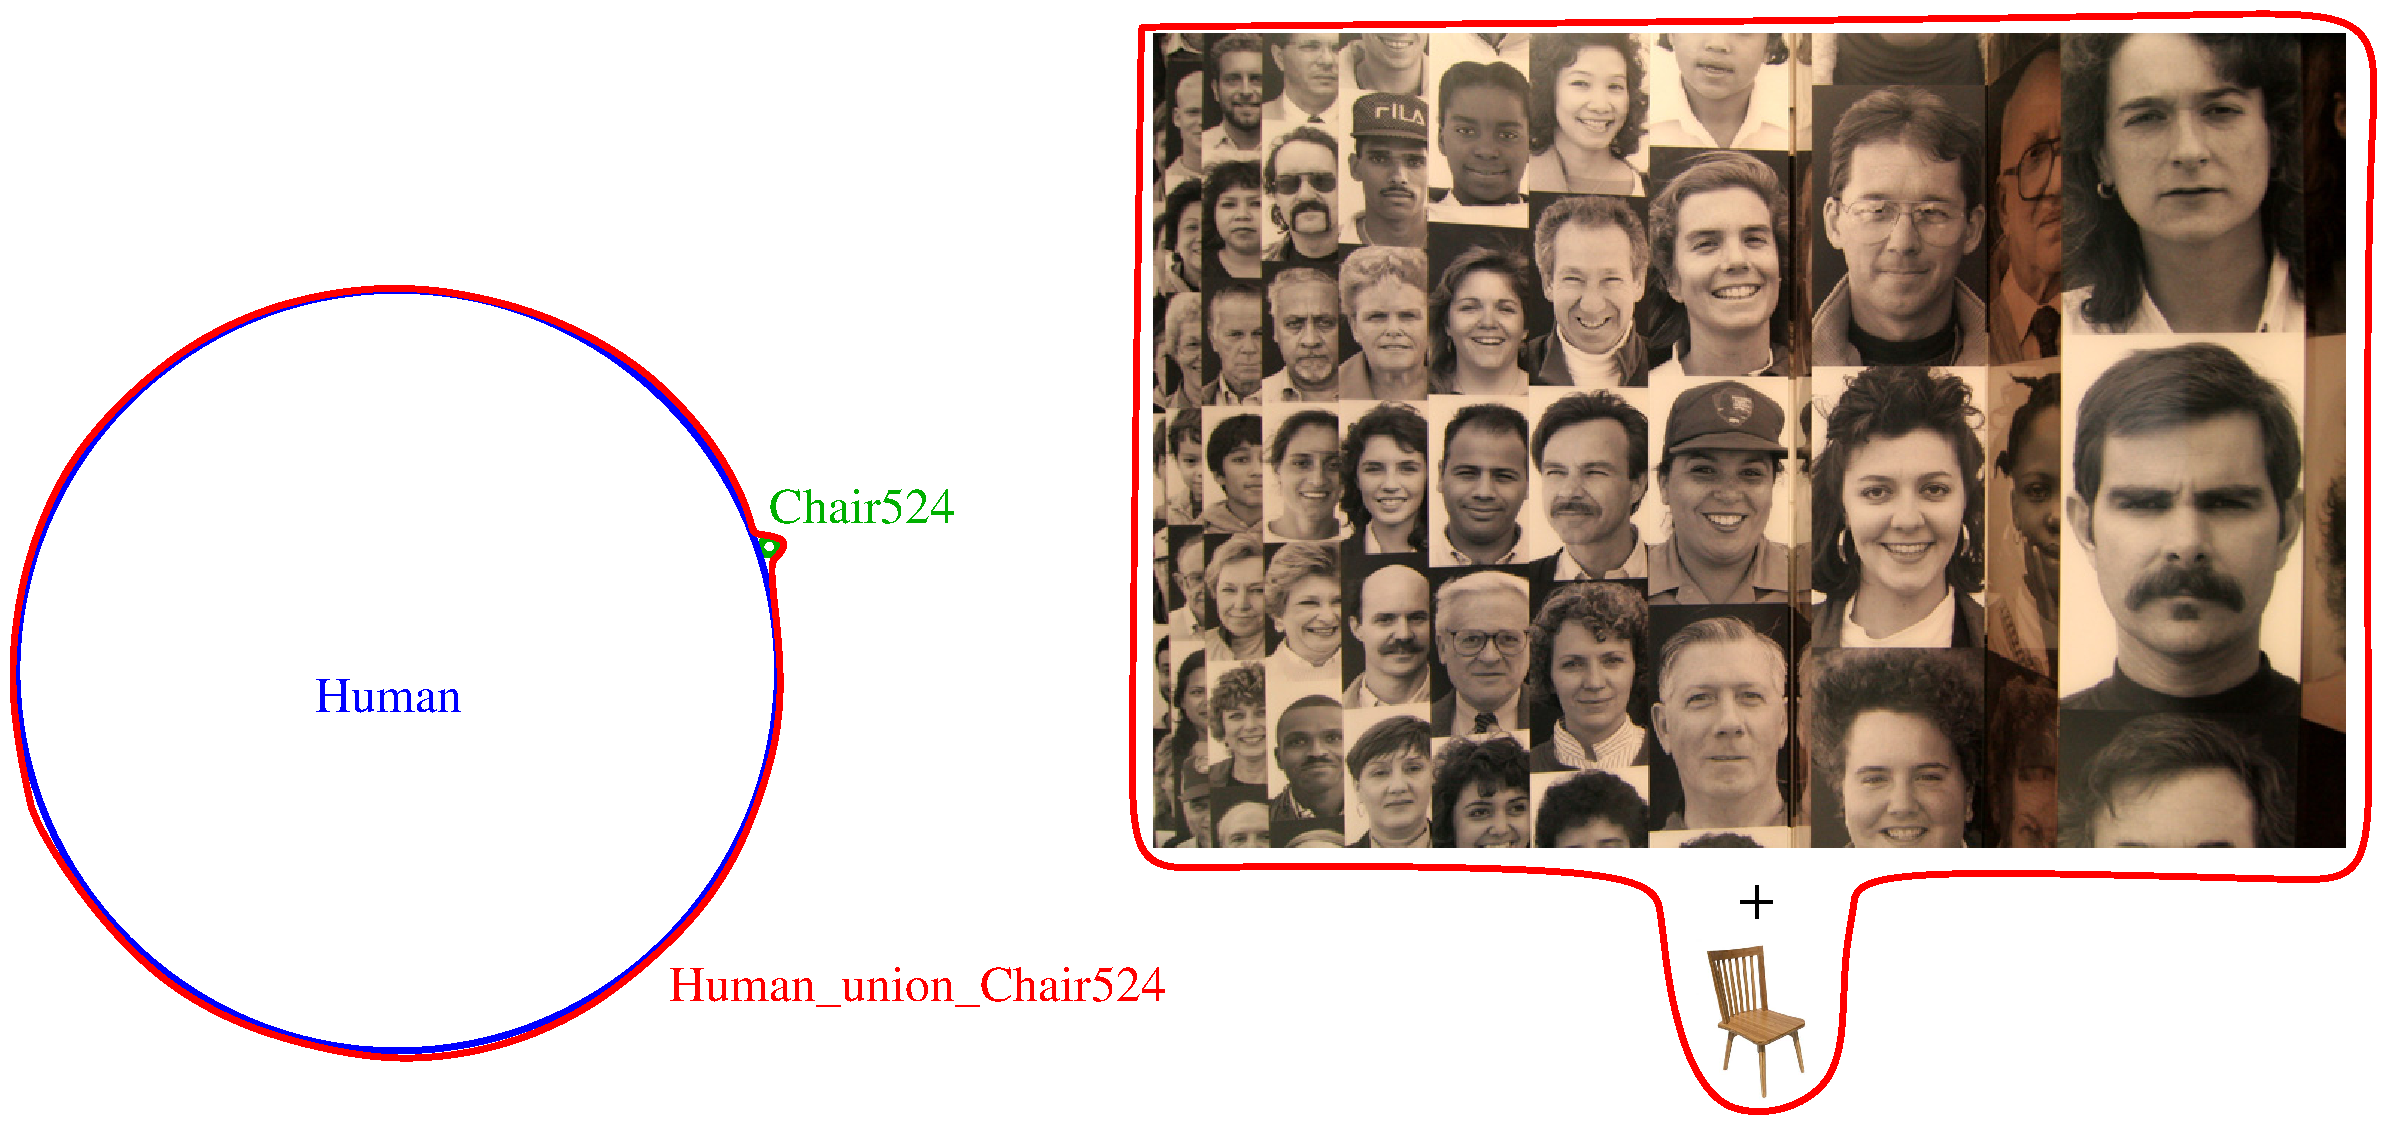
\includegraphics[scale=0.25]{human_chair_pic.pdf}}

  \visible<4>{
    \alert{$ASSOC(Human\_union\_Chair524,Human)$ is high},
    yet $Human\_union\_Chair524$ is \alert{not an interesting property}
    of Human.
  }
}

\frame
{
  \frametitle{Interesting property: \alert{Less complex} than the term itself}
  
  \begin{center}
    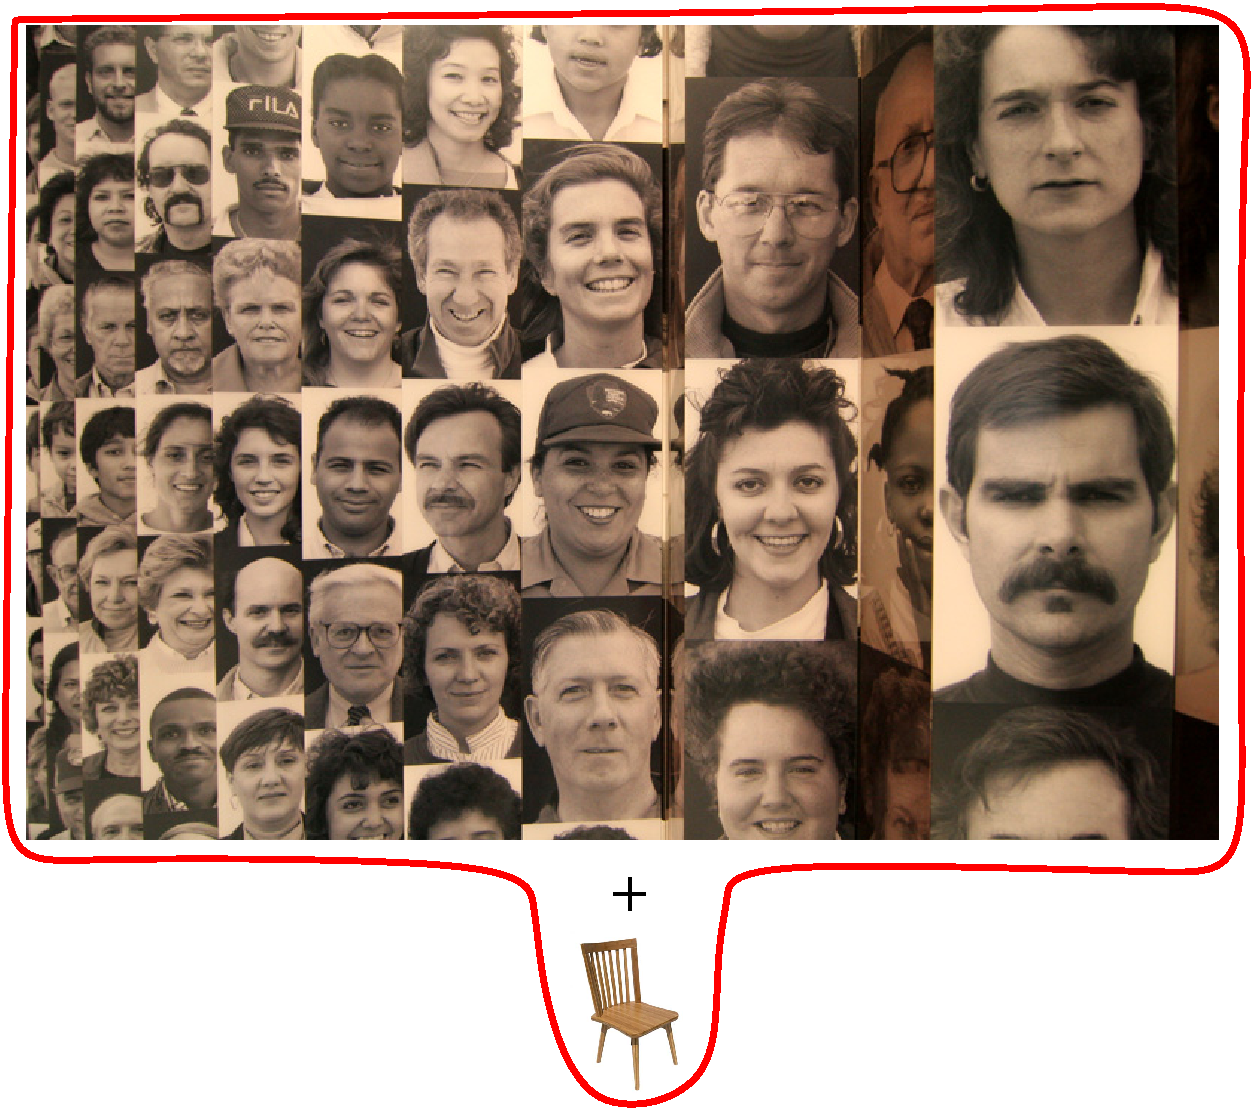
\includegraphics[scale=0.23]{hc_pic.pdf}
  \end{center}

  \begin{beamerboxesrounded}{$Human\_union\_Chair524$ is
      \alert{more complex} than Human}
    $c(Human\_union\_Chair524) \approx c(Human) + c(Chair524)$
  \end{beamerboxesrounded}
}

\frame
{
  \frametitle{Interesting property: \alert{Less complex} than the term itself}

  \begin{center}
    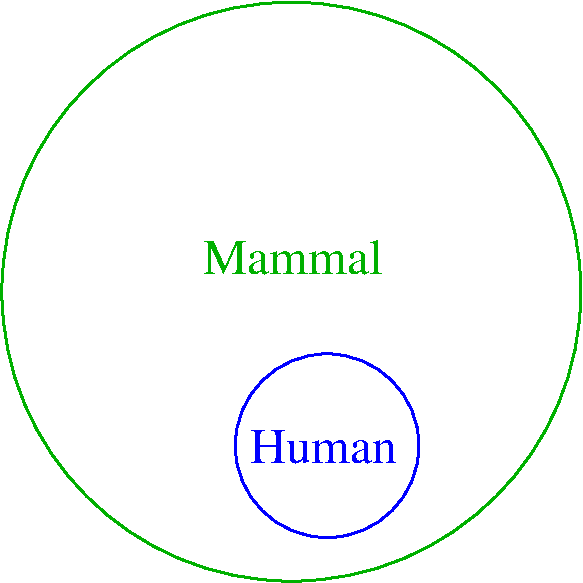
\includegraphics[scale=0.4]{mammal_human.pdf}
  \end{center}
  
  \begin{beamerboxesrounded}{Mammal is \alert{less complex} than Human,
      c(Mammal) < c(Human)}
    A human is a mammal + additional characteristics 
  \end{beamerboxesrounded}
}

\frame
{
  \frametitle{Interesting property: \alert{Less complex} than the term itself}

  \begin{beamerboxesrounded}{If $F$ is a property of $G$ we want}
    c(F)<c(G)
  \end{beamerboxesrounded}

  \[[c(G)-c(F)]^+\]
  \visible<+->{
  \visible<2->{Examples:}
  \begin{itemize}
  \item<+-> $[c(Human)-c(Human\_union\_Chair524)]^+ = 0$
  \item<+-> $[c(Human)-c(Mammal)]^+ > 0$\\[3ex]
  \end{itemize}
  }
  {\footnotesize Complexity of $F$, $c(F)$ is for example the
  shortest description of $F$ in some language $L$.}

}

\frame
{
  \frametitle{What is an \alert{interesting} property? A \alert{Pattern}}

  \begin{enumerate}
  \item Help \alert{differentiate} that term, $ASSOC(F,G)$\footnote{
      $ASSOC(F,G) = [P(F|G)-P(F|\lnot G)]^+$}

  \item \alert{Less complex} than the term itself,
    $[c(G)-c(F)]^+$
  \end{enumerate}
    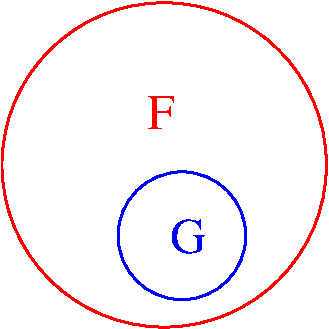
\includegraphics[scale=0.2]{F_G.pdf}  
  \pause

  \begin{beamerboxesrounded}{$F$ is a \alert{pattern} of $G$ if}
    $F$ is \alert{associated} with $G$ and $F$ is \alert{less complexe} than $G$
  \end{beamerboxesrounded}


    \[PAT(F,G)=[c(G)-c(F)]^+ \times ASSOC(F,G)\]
    
}

\frame
{
  \frametitle{Intensional Inheritance = Pattern Inheritance}

  \begin{beamerboxesrounded}{$A$ Intensionally Inherits $B$}
    \alert{How many patterns} $A$ inherits from $B$
  \end{beamerboxesrounded}
  
  \pause
  
  More formally...\\[2ex]

  Definition: $X\_PAT$ is the \alert{fuzzy set of all patterns of $X$}, that is:
  \[X\_PAT(G) = PAT(G,X)\]
 
  \pause
  
  For example:
  $
  \begin{array}{|lcc|}
    \hline
    Tiger\_PAT(Predator) & = & 0.3\\
    Tiger\_PAT(Mammal) & = & 0.4\\
    Tiger\_PAT(Carnivore) & = & 0.2\\
    Tiger\_PAT(Facing\_extinction) & = & 0.15\\
    Tiger\_PAT(Striped) & = & 0.3\\
    \hline
  \end{array}
  $
}

\frame
{
  \frametitle{Intensional Inheritance $\Rightarrow$ Extensional Inheritance}
  
  \begin{center}
    {\tt IntInh A B} $\ \ \equiv \ \ $
    {\tt ExtInh A\_PAT B\_PAT}\\
    $\equiv$\\
    {\tt SubSet A\_PAT B\_PAT}
    $\ \ = \ \  P(B\_PAT|A\_PAT)$
  \end{center}
}

\frame
{

  \frametitle{Intensional Inheritance $\Rightarrow$ Extensional Inheritance}

  For example: {\tt IntInh Tiger Lion <?>}

  \pause 

  \begin{enumerate}
  \item<+-> Determine Tiger\_PAT and Lion\_PAT

    \begin{columns}
      
      \column{1.5in}
      {\tiny
        $
        \begin{array}{|lcc|}
          \hline
          Lion\_PAT(Predator) & = & 0.3\\
          Lion\_PAT(Mammal) & = & 0.4\\
          Lion\_PAT(Carnivore) & = & 0.2\\
          Lion\_PAT(Facing\_extinction) & = & 0.1\\
          Lion\_PAT(Striped) & = & 0\\
          Lion\_PAT(Large\_Mane) & = & 0.3\\
          \hline
        \end{array}
        $
      }

      \column{1.5in}      

      {\tiny
        $
        \begin{array}{|lcc|}
          \hline
          Tiger\_PAT(Predator) & = & 0.3\\
          Tiger\_PAT(Mammal) & = & 0.4\\
          Tiger\_PAT(Carnivore) & = & 0.2\\
          Tiger\_PAT(Facing\_Extinction) & = & 0.15\\
          Tiger\_PAT(Striped) & = & 0.3\\
          Tiger\_PAT(Large\_Mane) & = & 0.01\\
          \hline
        \end{array}
        $
      }
      

  \end{columns}

  \item<+->

    {\tiny
      \begin{eqnarray*}
        P(Tiger\_PAT|Lion\_PAT)
        &
        =
        &
        \frac{\sum_x \min(Lion\_PAT(x), Tiger\_PAT(x))}
        {\sum_x Lion\_PAT(x)}\\
        \pause
        &
        =
        & 
        \frac{0.3+0.4+0.2+\min(0.1,0.15)+\min(0,0.3)+\min(0.3,0.01)}
        {0.3+0.4+0.2+0.1+0+0.3} = 0.78
      \end{eqnarray*}
    }

  \item<+->
      \alert{{\tt IntInh Lion Tiger <0.78>}}
  \end{enumerate}

}

\section{Conclusion}

\frame
{
  \frametitle{Conclusion}
  \begin{itemize}
  \item<+-> {\tt ExtensionalInheritance A B <p>} $\ \equiv\ P(B|A)=p$
  \item<+-> A\_PAT is the fuzzy set of \alert{interesting properties} of A,
    called \alert{patterns}
  \item<+-> {\tt IntensionalInheritance A B <p>}\\
    $\ \ \ \ \ \ \ \ \ \ \ \ \ \ \ \ \ \ \ \ \ \ \ \ \equiv$\\
    {\tt ExtensionalInheritance A\_PAT B\_PAT <p>}
  \end{itemize}
    
}

\end{document}
